\section{Introduction}

\begin{frame}
	\frametitle{Challenging Problem}
	
	\begin{center}
		\begin{tikzpicture}
			\node at (0,0) [draw=white,ultra thick,inner sep=0pt]
			{
				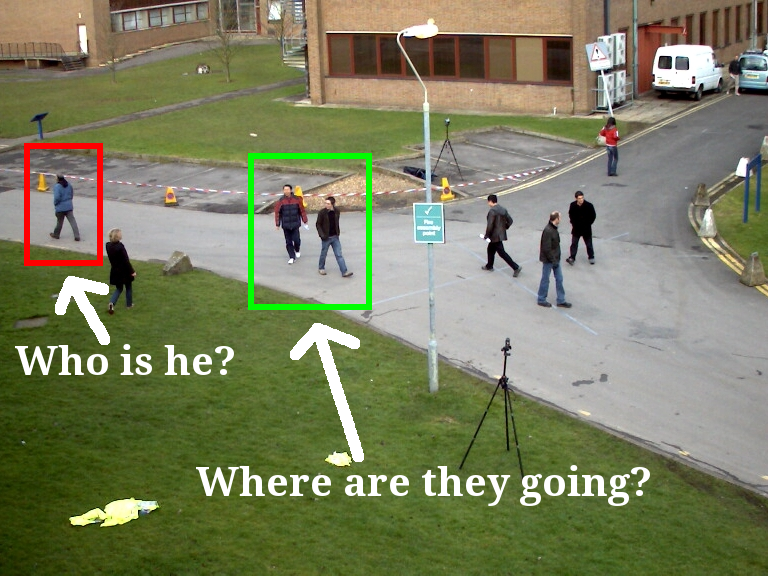
\includegraphics[width=\linewidth]{Figures/Problem.png}
			};
		\end{tikzpicture}
	\end{center}
\end{frame}

\begin{frame}
	\frametitle{Motivation}
	
	\vspace{0.2cm}
	
	\Large
	
	\begin{block}{Objective}
		\textbf{Understanding} the concept of human preference \textbf{allows} to perform higher levels
		of reasoning about future human actions. Likewise, the \textbf{knowledge} of a goal also gives
		information about \textbf{what} a person might do
	\end{block}
	
	\vspace{0.3cm}
	
	Example of application fields:
	\begin{itemize}
		\item Automatic video surveillance
		\item Human-Robot Interaction
		\item Domestic robots
	\end{itemize}
\end{frame}

\begin{frame}
	\frametitle{Contributions}
	
	\Large
	
	The main contributions of this thesis are:
	
	\begin{enumerate}
		\item \textbf{Distributed real-time} multiple object tracking
		\item \textbf{Asynchronous} and \textbf{fully} scalable design
		\item \textbf{Prediction} without prior scene semantics knowledge
		\item \textbf{Incremental} updates of the \emph{IRL} model over time
		\item \textbf{Non-uniform grids} for representing world state
		\item \textbf{Efficient} and \textbf{scalable} solution for on-robot implementation
	\end{enumerate}
\end{frame}

\begin{frame}
	\frametitle{Proposed Solution}
	
	\vspace{0.5cm}
	
	\begin{tikzpicture}
		\node at (0,0) [draw=white,ultra thick,inner sep=0pt]
		{
			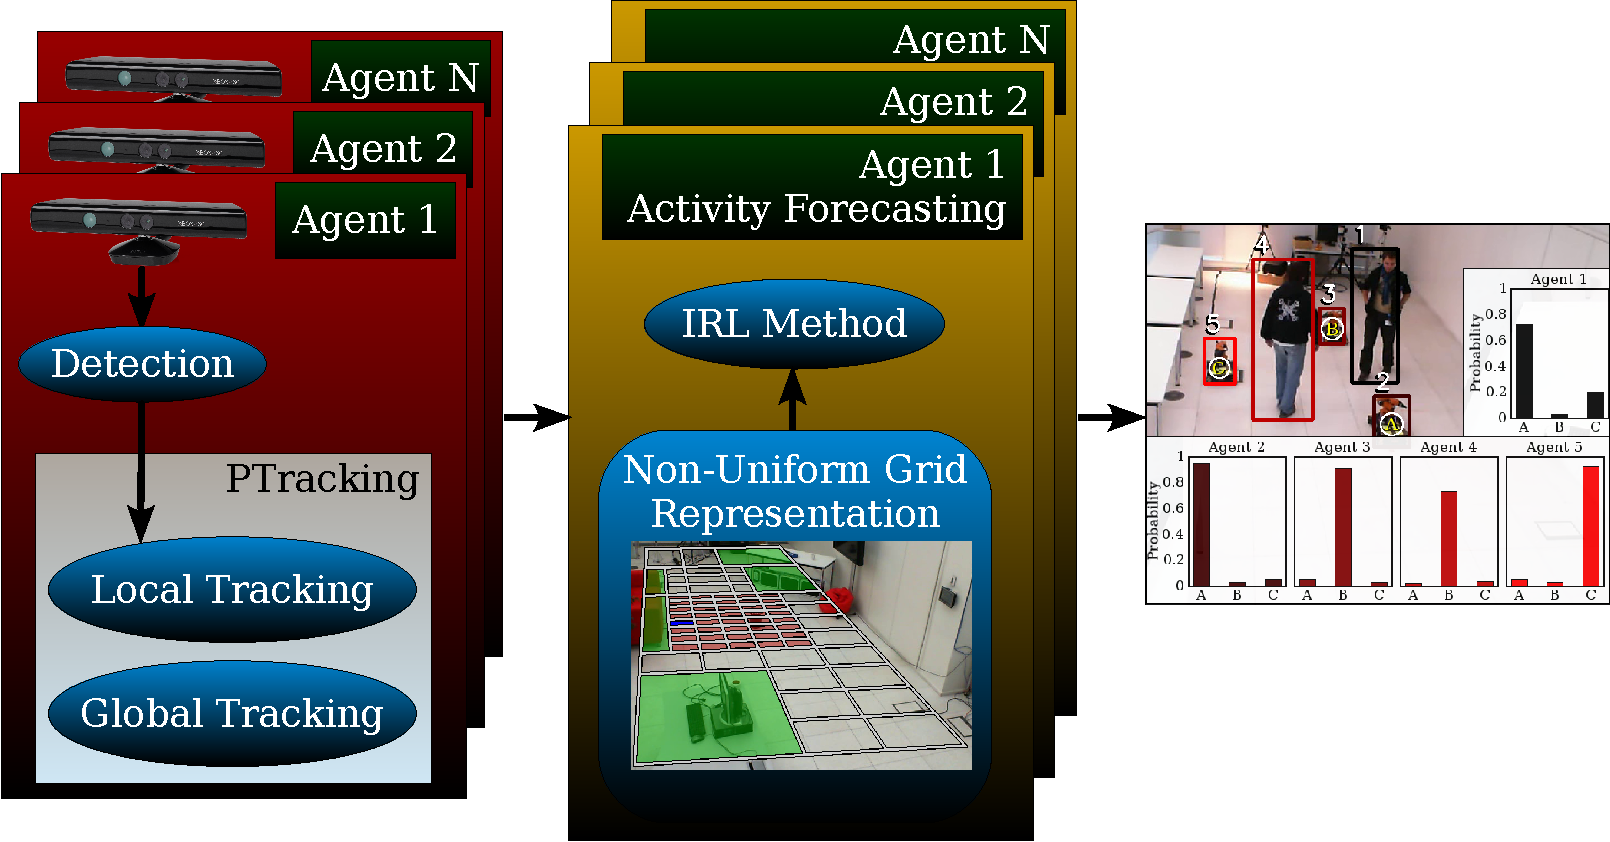
\includegraphics[width=\linewidth]{Figures/Architecture}
		};
	\end{tikzpicture}
\end{frame}
